\newpage

\section{Congruence via Transformations}
Two figures are said to be congruent if there exists a basic rigid motion (translation, 
rotation, or reflection) or a sequence of basic rigid motions that maps one figure onto 
the other.  (Note that typical definitions of congruence rely on measures of 
angles and sides, which works for polygons, but not more general figures.)  

\begin{prob}
One of the pairs of figures below shows a translation, and the other pair does not.  To identify which is which, draw segments between each point and its image.  Use those segments to explain your reasoning.
$$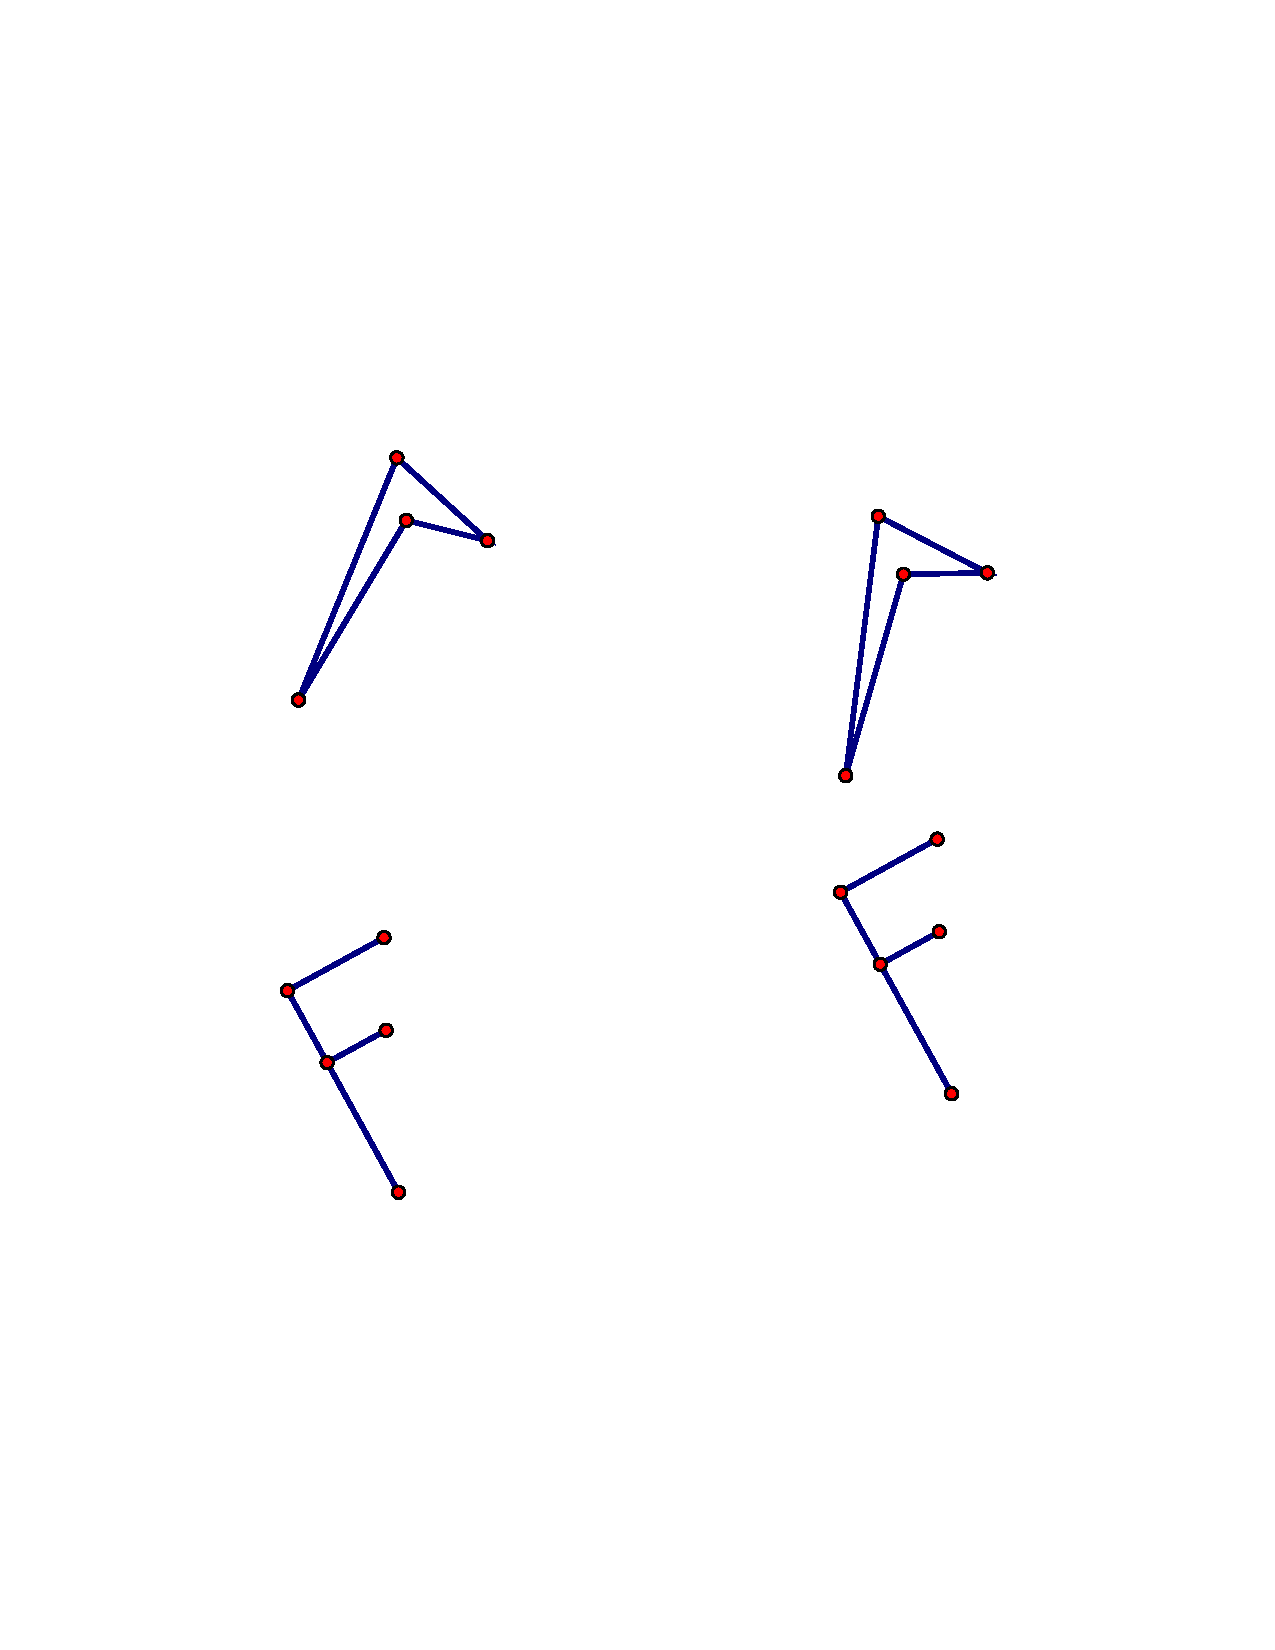
\includegraphics[scale=0.8]{../graphics/translate.pdf}$$
\end{prob}

\newpage

\begin{prob}
One of the pairs figures below shows a rotation about point C, and the other pair does not. 
\begin{enumerate}
\item Identify which pair of figures show a rotation about C, and explain how you know.  
\item Find the angle of rotation.  
\item Find the center of and angle of rotation for the other pair of figures.  Explain your reasoning.  
$$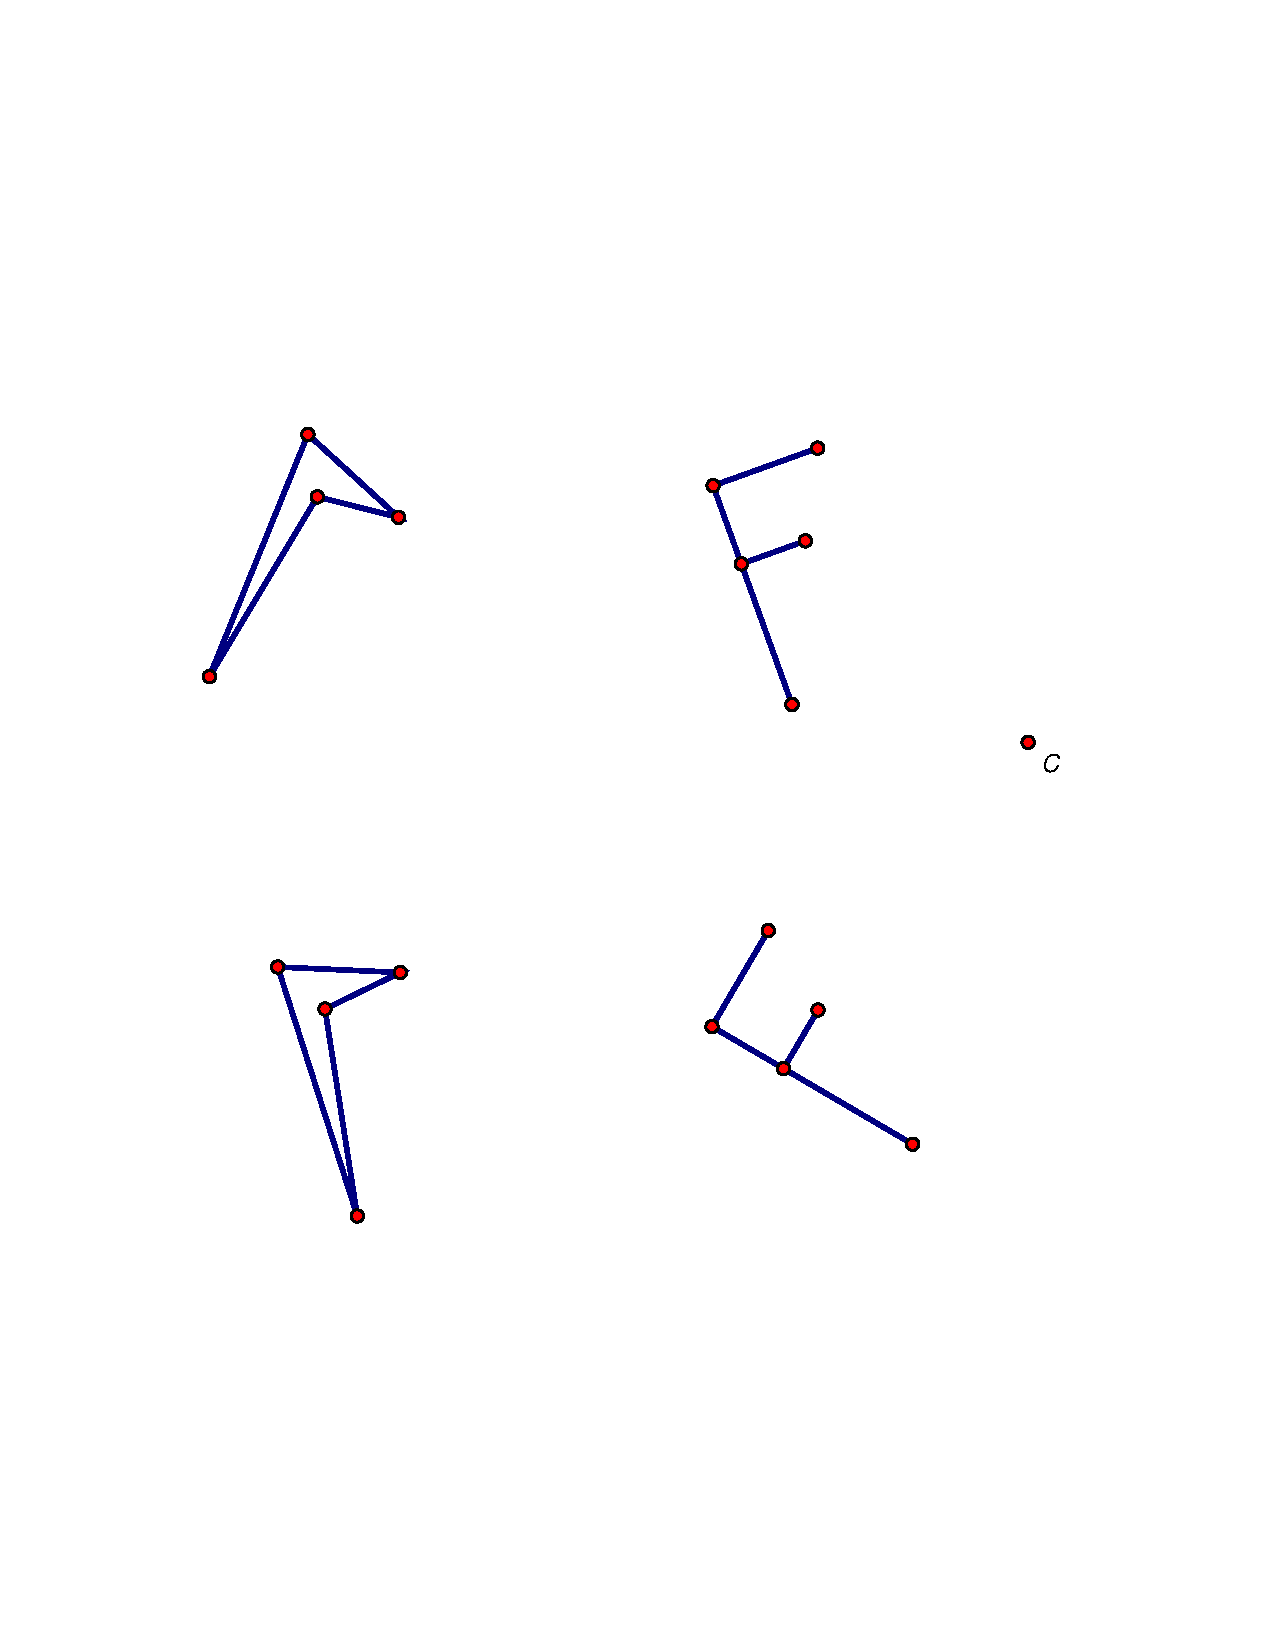
\includegraphics[scale=0.8]{../graphics/rotate.pdf}$$
\end{enumerate}
\end{prob}

\newpage
\begin{prob}
One of the pairs of figures shows a reflection about the given line, and the other pair does not.  
\begin{enumerate}
\item Identify which pair figures show a reflection about the given line, and explain how you know. 
\item Find the line of reflection for the other pair of figures, and explain your reasoning.  
$$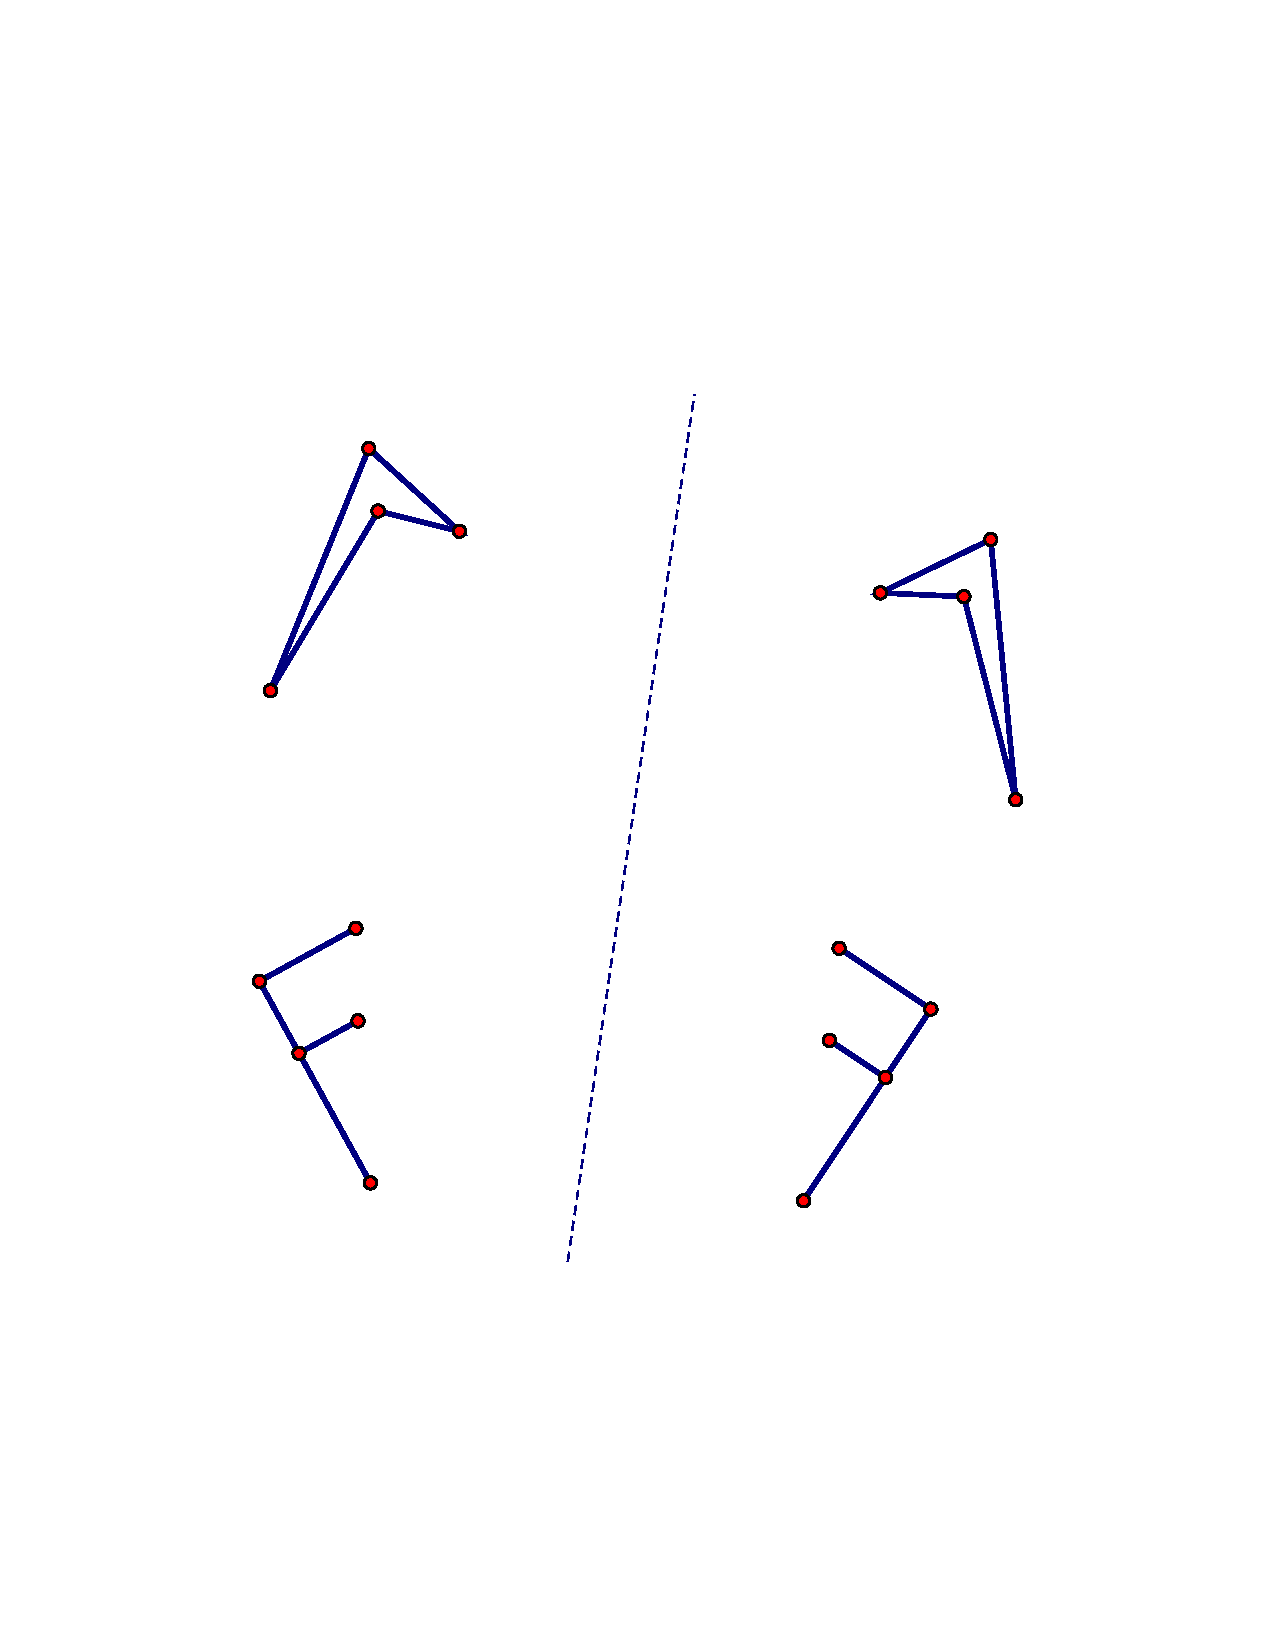
\includegraphics[scale=0.8]{../graphics/reflect.pdf}$$
\end{enumerate}
\end{prob}

\newpage
\begin{prob}
For the figures below, we want to identify a sequence of two or three basic rigid motions that takes one F onto the other.  Possibilities include a rotation followed by a translation or a reflection followed by a rotation. 
\begin{enumerate}
\item Explain briefly why, for this pair of figures, we can quickly exclude sequences of the following types: 
\begin{itemize}
\item a rotation followed by a rotation
\item a translation followed by a translation
\item a reflection followed by a reflection
\end{itemize}
\item Using tracing paper to illustrate intermediate images, identify a sequence of basic rigid motions that takes one F onto the other.  Explain your reasoning.  
\end{enumerate}
\vspace{1in}
$$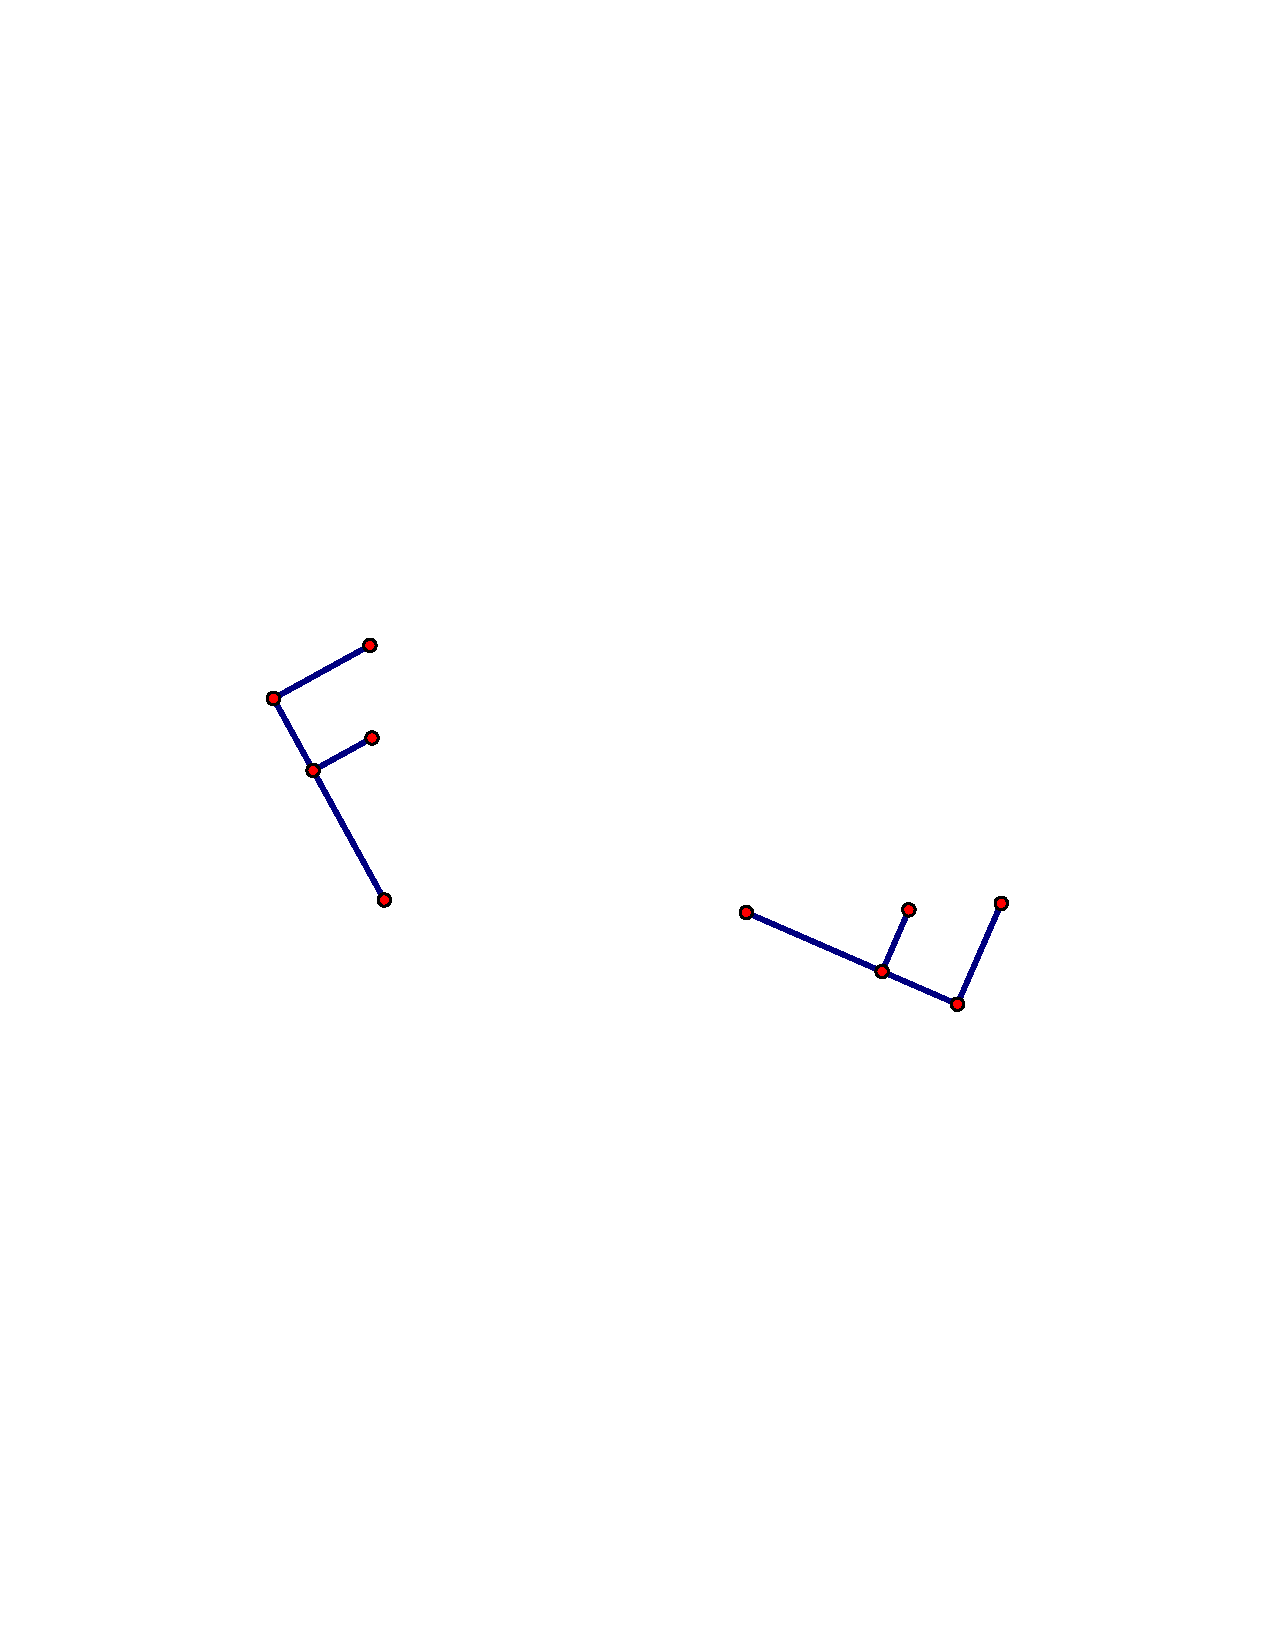
\includegraphics[scale=0.8]{../graphics/glideReflect.pdf}$$
\end{prob}

